\chapter{Introduction}

Rapid situational awareness is crucial to enabling a successful response from first responders during an emergency. Incident command uses all information available to them to make decisions and coordinate the first responders. First responders are often sent into the incident scene to gather information, but the nature of emergencies makes this process dangerous and can risk additional lives \cite{whysubtmatters}. Subterranean environments pose a number of additional hazards and challenges, such as outdated maps, dangerous terrain, and low visibility, making them particularly difficult to send humans into safely. For example, emergency personnel cannot safely explore beyond fires in coal mines, and are thus unable to determine the number of people or quality of terrain that may be behind them \cite{mshapresentation}. Autonomous systems have the potential to significantly improve the quality and timeliness of the situational awareness gained in challenging subterranean environments, and by doing so can reduce risk to human lives.

\section{The DARPA Subterranean Challenge (SubT)}

The DARPA (Defense Advanced Research Projects Agency) Subterranean Challenge was issued to spur the development of new technologies for exploring complex underground environments. Teams are challenged to propose new and innovative solutions for the unique perception, mobility, communication, and autonomy problems present in these environments. Teams compete in a series of 3 separate circuit events, each in a different type of subterranean environment, listed in Figure \ref{darpa_environments}. The highest performing teams will be invited to a final event which incorporates elements of each type of environment. In each event, teams are tasked with deploying systems which rapidly provide situational awareness, in the form of map data and locations of predetermined objects placed by DARPA. Each object ("artifact") represents a particular class of objects which are likely to be found in subterranean environments, such as those shown in Figure \ref{tunnel artifacts}.

\begin{figure}	
	\centering
	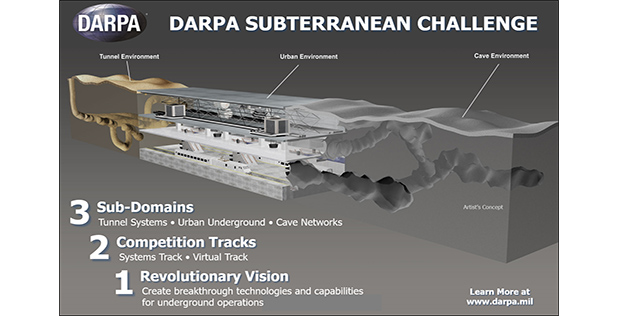
\includegraphics[width=\textwidth]{darpa_environments.jpg}
	\caption[DARPA Subterranean Challenge environments]{The Tunnel Circuit focuses on human made tunnel systems. The Urban Circuit focuses on urban environments such as mass transit and municipal infrastructure. The Cave Circuit focuses on naturally occurring cave systems. Image from DARPA \cite{subtenvironments}.}
	\label{darpa_environments}
\end{figure}

During each circuit event, teams have 60 minutes to deploy their systems in the environment. The deployment may consist of as many robots as the teams desire, but must be operated by a single human supervisor at the team's base station. Not all areas of the environment will be traversable for all types of robots, so teams are encouraged to develop systems with a variety of mobility capabilities. Autonomous exploration capability is advised to reduce operator load and eliminate a need for constant connectivity. Communication with and coordination of each robot in the fleet is a challenge as no communication infrastructure is provided by DARPA.  The perception systems used to drive the autonomy should be able to handle a variety of challenging conditions, such as low visibility and variable lighting. This differs from typical perception benchmarks, such as ImageNet \cite{deng2009imagenet}, which ensure clean and high quality data. Teams may be permitted multiple runs per event.

Before a team's run, DARPA places a predetermined and disclosed number of artifacts in the environment. The locations of specific points on each of these artifacts, referenced to a DARPA-defined frame, are surveyed and treated as ground truth. The location of each artifact and number of each artifact type is unknown to teams. Scoring for each competition event is based entirely on the number of artifacts which are correctly reported to DARPA within the 60 minute period. Teams must report the artifact's category and must report coordinates which are within 5m Euclidean distance of the ground truth for an artifact report to be considered correct. Teams may submit twice the number of artifact reports as there are artifacts in the environment. Artifact reports may be generated in whichever manner a team deems appropriate, such as randomly, by the human supervisor, or fully autonomously by the deployed system. Ties between multiple teams are broken by a number of factors, including the times artifacts were submitted, and the furthest artifacts detected \cite{tunnel_rules}.

\section{Tunnel Circuit Specifics}

This work focuses specifically on artifact detection and localization in the context of the Tunnel Circuit. The Tunnel Circuit event took place between at the National Institute for Occupational Safety and Health Mining (NIOSH) site in Pittsburgh, PA, between August 15 and August 22 2019. DARPA divided the former coal mine into two separate courses, starting at the mine's two separate portals, Safety Research and Experimental. A map of the Safety Research course is shown in Figure \ref{tunnel_circuit_day_2}. Each team was allowed 2 runs in each course. The team's final score is a sum of the highest score from each course.

20 artifacts were deployed by DARPA in each course. The placement and distribution of artifacts varied between each course and each run, as indicated in Table \ref{final_scores}. Five specific categories of artifacts were used at the Tunnel Circuit. A single representative model of each artifact, shown in Figure \ref{tunnel artifacts}, was used. Specific model numbers for each representative object were distributed to teams in advance of the competition \cite{tunnel_artifacts}.

\subsubsection{Backpack}

The backpack artifact represents a typical adult-sized bag for carrying items. The backpack may be found on the ground, on a wall, or resting on a work surface, such as a table. The backpack contains a sandbag to help keep it in place during the competition. The front backpack is facing outward or upward depending on the initial placement.

\subsubsection{Cell Phone}

The cell phone artifact represents a radio used for communication, as well as other typical handheld devices. The cell phone is playing an unspecified full-screen video. Audio is playing from the phone at maximum volume. A 2.4 GHz access point is created by each cell artifact with an SSID of the form "PhoneArtifact\#\#", where "\#\#" is a unique two digit number. The cell phone's Bluetooth radio is on and discoverable.

\subsubsection{Drill}

The drill artifact represents a typical handheld tool. The drill has a Philips head driver in its chuck. The artifact may be found on the ground or on work tables. The orientation of the drill is not specified. The drill is not powered during scored runs.

\subsubsection{Fire Extinguisher}

The fire extinguisher artifact represents a typical common handheld fire extinguisher. This artifact also represents areas where other emergency equipment may be located. The fire extinguisher has its hose in the stored configuration. It may be found on the ground, on a work surface, or hanging from a wall. It will not be used during the scored runs.

\subsubsection{Survivor ("Randy")}

The survivor artifact represents a human survivor, such as a trapped worker. A thermal manikin is used, and is wearing a high visibility jacket, work pants, and standard steel toed work boots. The manikin has heating elements in its hands and head to partially emulate a human's thermal signature. The manikin is not actuated and does not play auditory clues. The manikin is placed in a static sitting position against walls.

\begin{figure}
	\centering
	\begin{subfigure}{0.32\textwidth}
		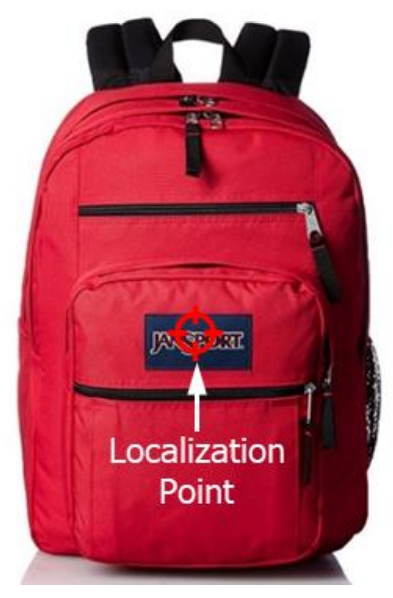
\includegraphics[width=\textwidth,height=5.5cm,keepaspectratio]{backpack_artifact.png}
		\caption{Backpack}
		\label{backpack}		
	\end{subfigure}
	\hfill
	\begin{subfigure}{0.32\textwidth}
		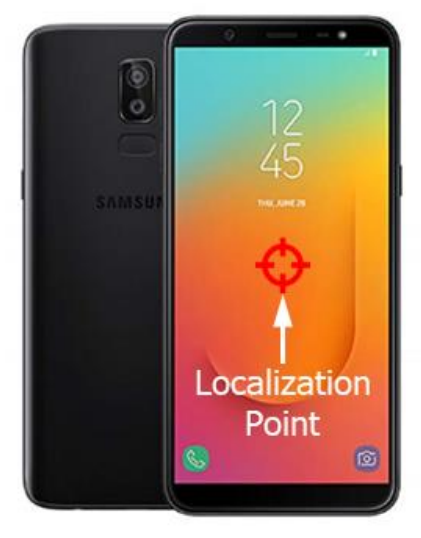
\includegraphics[width=\textwidth,height=5.5cm,keepaspectratio]{cell_phone_artifact.png}
		\caption{Cell Phone}
		\label{cell phone}
	\end{subfigure}	
	\hfill
	\begin{subfigure}{0.32\textwidth}
		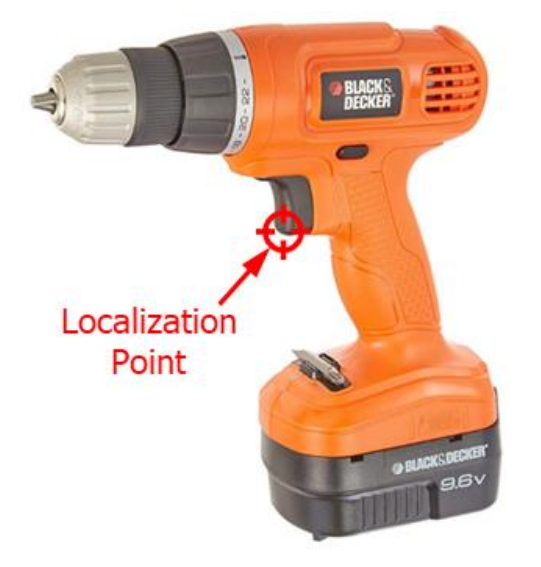
\includegraphics[width=\textwidth,height=5.5cm,keepaspectratio]{drill_artifact.png}
		\caption{Drill}
		\label{drill}
	\end{subfigure}
	\\
	\begin{subfigure}{0.32\textwidth}
		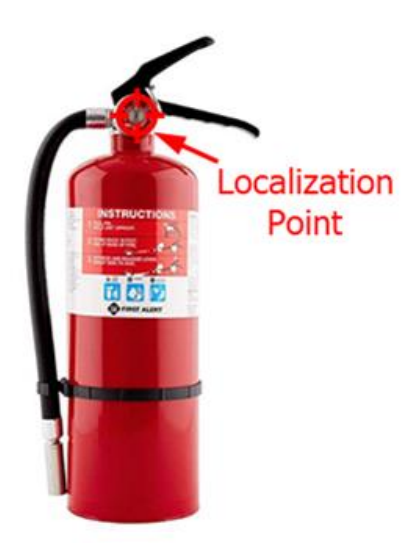
\includegraphics[width=\textwidth,height=5.5cm,keepaspectratio]{fire_extinguisher_artifact.png}
		\caption{Fire Exraaktinguisher}
		\label{fire extinguisher}
	\end{subfigure}
	\begin{subfigure}{0.32\textwidth}
		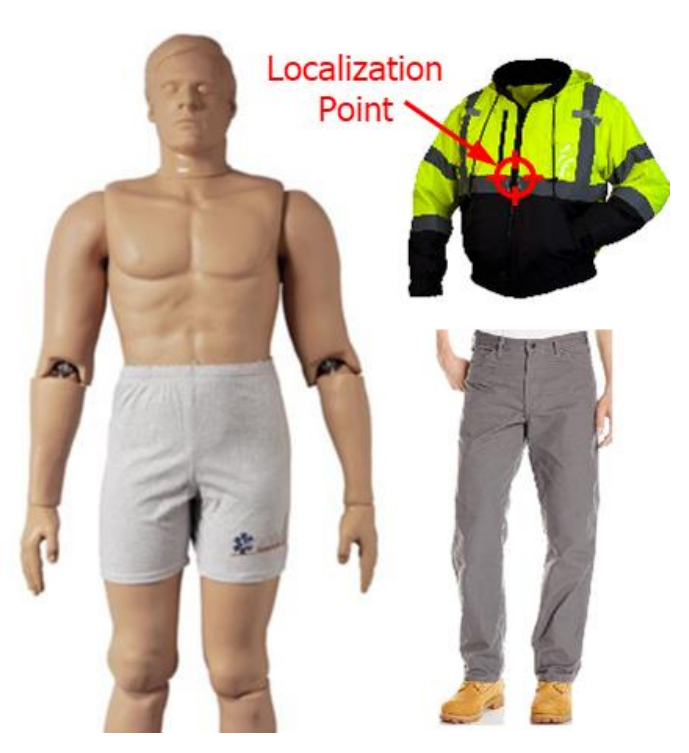
\includegraphics[width=\textwidth,height=5.5cm,keepaspectratio]{randy_artifact.png}
		\caption{Survivor ("Randy")}
		\label{randy}
	\end{subfigure}	
	\caption[Tunnel Circuit artifacts]{The Figure depicts the 5 Tunnel Circuit artifacts. The survivor, cell phone, and backpack artifacts are common to all 3 circuit events. Each circuit consists of an additional 2 circuit-specific artifacts, which were the fire extinguisher and drill for the Tunnel Circuit. All 9 artifacts will be used during the final event. The localization point in the images is the specific point surveyed by DARPA against which error will be measured. Images from DARPA \cite{tunnel_artifacts}.}
	\label{tunnel artifacts}
\end{figure}

\section{Our Approach}

Our team's overall concept of operations is one of modular autonomy. We aim to develop a set of hardware and software components that can be rapidly reconfigured and adapted to support the needs of any particular environment. Individual modules can be upgraded or replaced as necessary. For mobility, modules such as removable battery packs, wheel assemblies, and drive electronics are used. These mechanical modules combined to form 3 robots during the Tunnel Circuit -- R1, a fixed body ground robot, R2, a ground robot with a center pivot body, and D1, a hexcopter. For communication, custom nodes are developed, multiples of which can be stored on modular node dropper assemblies. R1 and R2 each carried a node dropper during the Tunnel Circuit. For perception, this approach means the development of various sensing payloads with integrated software and computation that can be transferred between robots. These sensing payloads run modular state estimation and artifact detection and localization software which can adapt to the capabilities of each system. R1, R2, and D1 each had separate sensing payloads -- Mk. 0, Mk. 1, and Drone payload, respectively.

Within each sensing payload, we use a multimodal suite of sensors for artifact detection. Though a single sensor or category of sensors, such as RGB cameras, may be able to detect multiple types of artifacts, it is unlikely to be able to perform well in all conditions. Alternatively, individual sensors may be particularly well suited to detect a specific artifact easily, but may not detect others at all. For example, the survivor and cell phone artifacts emit a thermal signature that may be able to be detected in a thermal camera, leading to the localization of these artifacts even in cases of little to no light. A WiFi radio may be used to detect and localize which is beyond line of sight, but is incapable of detecting any other categories of artifacts. Using a multimodal suite of sensors with intelligent fusion allows us to exploit the strengths of each individual sensor and create a more accurate and robust overall system.

The human supervisor is also considered a module in our system. Though each robot in the system is capable of autonomous operation, the human supervisor is able to combine course and map information reported from multiple robots and direct the exploration patterns of the fleet. Each robot also returns artifact information to the base station, which the human supervisor aggregates and verifies. Artifacts reports which have been approved by the human supervisor are sent to DARPA at the human supervisor's discretion, and are modified and resubmitted as more information becomes available if necessary. An overview of our approach is shown in Figure \ref{approach}.

\begin{figure}	
	\centering
	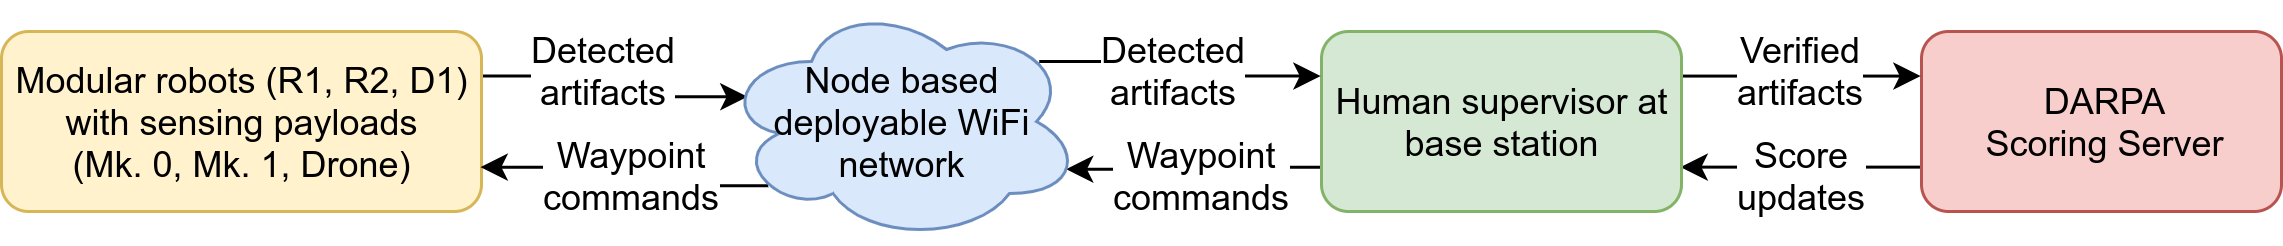
\includegraphics[width=\textwidth]{approach.png}
	\caption[Our approach]{Multiple robots explore the mine and deploy communication nodes as they go along. They report artifacts they detect to the human supervisor over the deployed network. The human supervisor verifies the artifacts and sends verified ones to DARPA. DARPA scores the artifacts and returns score updates. The human supervisor uses score updates, as well as other map information received from the robots, to guide autonomous exploration with waypoints.}
	\label{approach}
\end{figure}

\section{Related Work}

There has been relatively little recent work which addresses the complete problem of rapid situational awareness in subterranean environments, leading to the issuance of the DARPA SubT Challenge to develop new technologies in this space. However, many smaller components of the overall problem, such as single and multimodal object detection, modular sensing payloads, and object tracking are key research areas and have been well studied in other domains. This work draws inspiration from many of the state of the art techniques and technologies developed for other fields and applies and extends them for use in subterranean environments.

\subsection{Subterranean Mobile Robots}

The early 2000s saw the development of a number of robots intended for use in subterranean environments, such as CMU's Groundhog \cite{ferguson2004autonomous} and CSIRO's Numbat \cite{ralston1998numbat}. These robots were built to specifically address mobility and perception challenges presented by underground mines. They demonstrated considerable mobility in a variety of field experiments, but were limited in their autonomous capabilities by the available compute and sensing technologies \cite{morris2006recent}. They do not have the ability to provide rapid situational awareness to basestation operators, and the approaches used do not scale well to multiple robots.

Groundhog carries two scanning lasers for mapping and navigation, along with a gyroscope, encoders, and tilt sensors for odometry. 2D maps are generated on board and continually optimized to ensure global consistency, but are not reported to the base station due to a lack of communication infrastructure. The maps can be queried from recorded data after Groundhog returns. Though the fidelity of the maps is high enough to be useful for situational awareness, the high latency of the information (potentially multiple hours) can be costly in a disaster response scenario. Even after a base station operator downloads the maps from the robot, searching the point clouds for specific objects is a time consuming and inaccurate process when done manually.

The communication problem faced by Groundhog due to a lack of infrastructure was solved by other subterranean robots with a tether. This enabled robots, such as the MSHA (Mine Safety and Health Administration) Andros V-2, to report video feeds to the base station in real time. The remote camera acts as a source of more rapid situational awareness than the high latency point cloud maps from Groundhog, and provides data in a format more easily understandable by humans. However, tethers proved to be unreliable, being prone to tangling and breakage \cite{murphy2009mobile}, and thus unsuitable for disaster response scenarios which require robust solutions. Relying on streaming video for situational awareness is also difficult to scale due to the necessity of dividing the human operator's attention, potentially resulting in important data being missed.

The more recent MINBOT-II \cite{wang2014development} robot improves upon the tethered communication design with a controlled release fiber line, as well as adds multiple autonomy modes (semiautomatic and fully automatic) to reduce the burden on the human operator. Its tracked mobility design is inherently explosion- and water-proof, allowing for safe and reliable operation in mines. However, though MINBOT-II features more sensors than the Andros V-2 robot, including additional cameras and gas sensors, data is still displayed directly to the human operator without further postprocessing. This does not solve the fundamental issue of divided operator attention and difficult multi-robot scaling.

Our work addresses many of the limitations of previous autonomous systems for providing situational awareness. Each deployed robot in our system autonomously identifies important objects and sends it to the base station over a wireless link. Providing artifacts for situational awareness ensures that the human supervisor receives only high utility information, and reduces the difficulty of operating multiple robots covering a large environment at once. The small size of each artifact also enables transmission over a wireless link even when only low bitrates are available, ensuring real time updates.

\subsection{Modular Sensing Payloads}

A major contribution of our work is a collection of modular sensing payloads for robot mapping, autonomy, and perception. There are a number of academic and commercial projects which have developed payloads which are similar in spirit, though they focus primarily on 3D mapping and autonomy and do not offer on board high level perception algorithms. One such example is the Kaarta Stencil \cite{kaarta}, a SLAM-based 3D mapping payload capable of operating on both ground and aerial robots. It provides loop closed maps and pose information to the connected robot, and performs all compute on board. It can also be hand carried if desired, in which case it will store information on board for offline viewing and processing. 

A similar system is the Emesent Hovermap \cite{hovermap}, a mapping and autonomy payload specifically targeting industrial drones. The payload only uses a rotating LIDAR for its SLAM-based mapping, instead of both (fixed) LIDAR and RGB camera information like the Stencil does, but compensates by offering on board autonomy features instead. It is specifically advertised as being suitable for use in underground mines and other similar GPS-denied environments. Proximity to nearby obstacles is reported to the operator for situational awareness, along with live camera views. The complete 3D maps are only available after the drone has landed and brief offline postprocessing is applied.

The Zebedee Mobile Mapping System \cite{zlot2014three} is an academic system specifically targeting subterranean mapping in caves. The payload uses a fixed LIDAR mounted on a spring which helps extend the field of view of their selected planar LIDAR. Zebedee requires a separate computer and battery in addition to the payload, both of which are typically carried by a human in a backpack. Data from the LIDAR and IMU is recorded on the attached computer and processed offline to generate a 3D point cloud. Even with the processing time, data can be collected and visualized much more quickly than traditional approaches based on surveying and total stations, but at the cost of map resolution and accuracy. The compact and hand carried nature of the payload makes it usable in tight spaces that would be difficult for robots carrying payloads like the Stencil or Hovermap to access, but the necessity of a human operator prohibits its use in subterranean disaster response scenarios.

\subsection{2D RGB Object Detection}

2D object detection for RGB images has seen significant progress in recent years with the advent of deep learning and high quality datasets such as Pascal VOC \cite{everingham2010pascal} and COCO \cite{lin2014microsoft}. One of the first frameworks to deliver impressive performance was RCNN \cite{girshick2014rich}, which uses 2 distinct stages to detect bounding boxes around objects. RCNN generates multiple region proposals in the first stage, and extracts features from each one using a deep feature extractor (CNN) and uses an SVM to classify the generated features in the second stage. Running the CNN on each proposed region is computationally expensive and was improved upon by Fast RCNN \cite{girshick2015fast}, which primarily speeds on RCNN's inference speed by running the deep feature extractor once and then proposing regions from the feature map, instead of the other way around. It also replaces the SVM classifier with a softmax layer to consolidate all training into a single network. Faster RCNN \cite{ren2015faster} further improves upon the inference speed of Fast RCNN by replacing the selective search based region proposal with a regional proposal network that can be parallelized and run on a GPU, among other improvements.

Even with these improvements, Faster RCNN based detectors are too slow to run in real time on any but the most powerful systems. One stage object detection frameworks such as YOLO and SSD improved inference speed compared to Faster RCNN at the cost of some accuracy. Both YOLO \cite{redmon2018yolov3} and SSD \cite{liu2016ssd} eliminate the region proposal step and instead used a fixed number of multi scale bounding box priors which are adjusted and classified. The priors are then filtered to retain only ones which are highly likely to be objects. Training with the large number of boxes is difficult due to a class imbalance between positive and negative examples. RetinaNet \cite{lin2017focal} solves this problem by introducing a new loss function, focal loss, which weights the gradient based on the ease of classification. When combined with an efficient mobile-friendly feature extraction network such as MobileNet \cite{sandler2018mobilenetv2}, each of these object detection frameworks achieves impressive framerates on even modest hardware. Our payloads use object detection networks based on MobileNet and SSD to perform inference at camera framerate for multiple RGB cameras.

\subsection{RGB + Other Sensor Object Detection}

Some prior work exists related to object detection exclusively with non-RGB image-based sensors (e.g. thermal \cite{berg2016detection, nan2019infrared}), but is often limited by the lack of large datasets similar to those available for RGB. To overcome this, many approaches choose to utilize existing RGB datasets and networks in some way as a bootstrapping mechanism. \cite{devaguptapu2019borrow} uses two branches in its feature extraction network -- one operating directly on thermal images, and another operating on pseudo-rgb images generated by an image-to-image translation network with thermal image input. The pseudo-rgb branch is initialized with weights from a pretrained RGB detector. \cite{agrawal2019enhancing} performs joint detection on RGB and thermal image pairs, treating the thermal images as a fourth input channel. The Faster RCNN based network used is initialized with weights from pretraining on COCO. They show that the inclusion of thermal images improves object detection performance over the RGB-only baseline, with notable improvement in nighttime conditions.

Point cloud based object detection methods such as \cite{beltran2018birdnet, li2016vehicle} provide ways of utilizing 3D data for object detection, but suffer from the limited resolution available in modern LIDAR sensors. A variety of techniques to fuse LIDAR and RGB data for improved performance, as measured on datasets like KITTI \cite{Geiger2013IJRR}, have been proposed. Much of this work has been motivated by the need for self driving cars to accurately perceive their environments in all conditions \cite{feng2019deep}. \cite{qi2018frustum} performs 2D object detection in RGB images and then projects and refines detections into 3D using LIDAR information. \cite{liang2019multi} instead jointly extracts features from LIDAR and RGB camera data and performs ROI feature fusion to achieve state of the art performance on KITTI.

Unfortunately, though they achieve impressive accuracy, state of the art deep fusion techniques do not typically run in real time on constrained hardware. Many of the custom operations used by these networks are unavailable in optimized inference frameworks such as TensorRT and OpenVINO, resulting in either a complete inability to run the network or a fallback to slow reference implementations in other frameworks such as TensorFlow. Even disregarding the compute issues, field of view overlap is required for deep fusion, which is not the case between any pair of RGB and thermal cameras on Mk. 1. Furthermore, the precise sensor synchronization between either RGB and thermal images, or RGB images and LIDAR scans is missing in all of our payloads due to hardware limitations.